\documentclass[12pt,a4paper,oneside]{report}
\usepackage[T1]{fontenc}
\usepackage{lmodern}
\usepackage{amsmath}
\usepackage{graphicx}
\usepackage{booktabs}
\usepackage[margin=2.5cm]{geometry}
\usepackage{setspace}
\usepackage{hyperref}
\onehalfspacing

\begin{document}

\begin{titlepage}
  \centering
  \vspace*{2cm}
  {\LARGE\bfseries Urban Heat Islands and Vegetation Cover in Mid-Sized Cities\par}
  \vspace{2cm}
  {\large A thesis submitted in partial fulfilment of the requirements for the degree of\par}
  {\large Master of Science in Environmental Science\par}
  \vspace{2cm}
  {\Large Rosa Delgado\par}
  \vfill
  {\large Department of Geography\\University of Leeds\\September 2026\par}
\end{titlepage}

\begin{abstract}
This thesis examines the relationship between vegetation cover, measured by the
normalised difference vegetation index (NDVI), and land surface temperature in twelve
European cities of between 200\,000 and 800\,000 inhabitants.
\end{abstract}

\tableofcontents
\listoffigures
\listoftables

\chapter{Introduction}
\label{ch:intro}
Cities are warmer than their rural surroundings. This \emph{urban heat island} effect
increases energy demand and heat-related mortality. Chapter~\ref{ch:data} describes the
data and Chapter~\ref{ch:results} presents the results.

\section{Research questions}
\begin{enumerate}
  \item How strongly is NDVI associated with land surface temperature?
  \item Does the association vary with city size?
\end{enumerate}

\chapter{Data and Methods}
\label{ch:data}
\section{Satellite imagery}
We used Landsat 8 scenes acquired between June and August 2024. NDVI is defined as
\begin{equation}
\mathrm{NDVI} = \frac{\mathrm{NIR} - \mathrm{Red}}{\mathrm{NIR} + \mathrm{Red}}.
\end{equation}
Figure~\ref{fig:ndvi} shows an example NDVI map.

\begin{figure}[htbp]
  \centering
  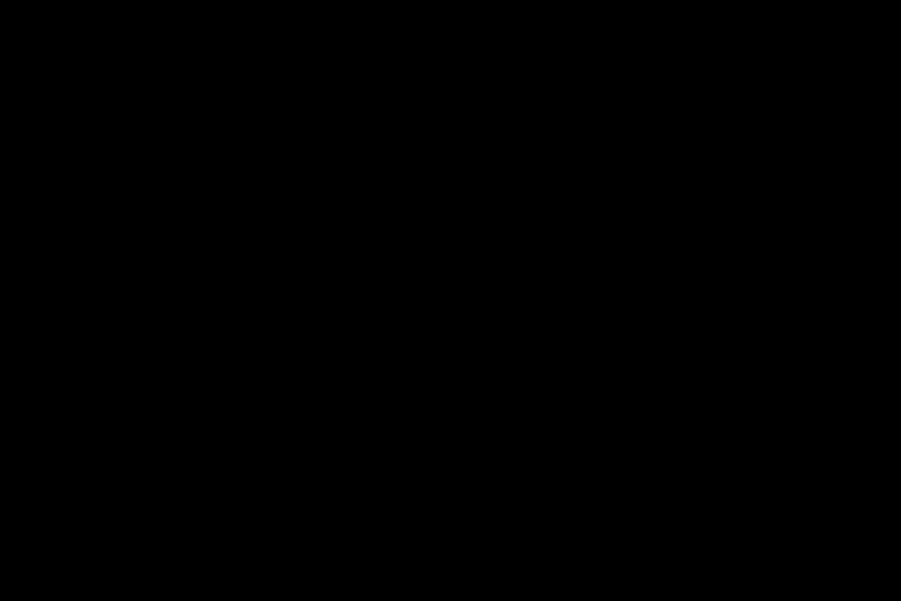
\includegraphics[width=0.7\textwidth]{ndvi-map.pdf}
  \caption{NDVI over the study area, July 2024.}
  \label{fig:ndvi}
\end{figure}

\section{Statistical model}
We fit a linear mixed model with a random intercept per city.

\chapter{Results}
\label{ch:results}
Table~\ref{tab:coef} summarises the fitted coefficients.

\begin{table}[htbp]
  \centering
  \caption{Fixed-effect estimates.}
  \label{tab:coef}
  \begin{tabular}{lrrr}
    \toprule
    Term & Estimate & SE & $p$ \\
    \midrule
    Intercept & 34.2 & 0.81 & $<0.001$ \\
    NDVI & $-8.7$ & 0.44 & $<0.001$ \\
    Population (100k) & 0.31 & 0.12 & 0.011 \\
    \bottomrule
  \end{tabular}
\end{table}

\appendix
\chapter{Scene List}
All Landsat scene identifiers are listed in the supplementary data.

\begin{thebibliography}{9}
\bibitem{oke} T.~R. Oke. The energetic basis of the urban heat island.
  \emph{Quarterly Journal of the Royal Meteorological Society}, 108(455):1--24, 1982.
\bibitem{weng} Q.~Weng, D.~Lu, and J.~Schubring. Estimation of land surface
  temperature--vegetation abundance relationship. \emph{Remote Sensing of Environment},
  89(4):467--483, 2004.
\end{thebibliography}

\end{document}
